\subsection{Problems to be addressed}
\label{subsec:problems-to-be-addressed}

In this section, I will outline the potential problems that I may encounter during our research and how I plan to address them.
Each problem is going to be presented as a subsection, with a brief description of the problem and how I plan to address it.

\subsubsection{How to measure memory usage}

One of the primary challenges in our research is accurately measuring memory usage.
This is particularly true for \ac{GPU} memory, which may differ from \ac{CPU} memory.
I aim to explore different options to measure memory usage accurately.

I plan to start by investigating if there is an API to measure \ac{GPU} memory consumption, and if not, I will explore common libraries that allow gathering memory consumption based on a specific process.
I understand that the optimal approach would be to use a specific API for this, since this would allow more flexibility for our tool, but I will explore alternative options if necessary.

\subsubsection{Historical data requirements}

Many of the current approaches require a significant amount of historical data to train the models.
This is not feasible for my research, as it would be time-consuming to generate such data for algorithm-specific models.
Also, even if I decide to generate such data, this would add a requirement for the user to have a significant amount of data to train the models for any new algorithm they want to use.

To overcome this limitation, I plan to implement a reinforcement learning approach to train the models.
This approach will allow the model to learn from the data while it is being used, learning from its own mistakes and improving its predictions.
Figure \ref{fig:reinf-learning} shows a diagram illustrating how this approach will work.
The memory estimator is going to act as the agent, using the input shape and other features as its state to generate a estimate of the memory usage.
A equality function will be used to compare the predicted memory usage with the actual memory usage, and this will be used to calculate the reward for the model.
Each execution of the algorithm will act as a round to train the model.

\begin{figure}[ht]
  \caption{Reinforcement learning execution diagram}
  \label{fig:reinf-learning}
  \resizebox{\textwidth}{!}{%
    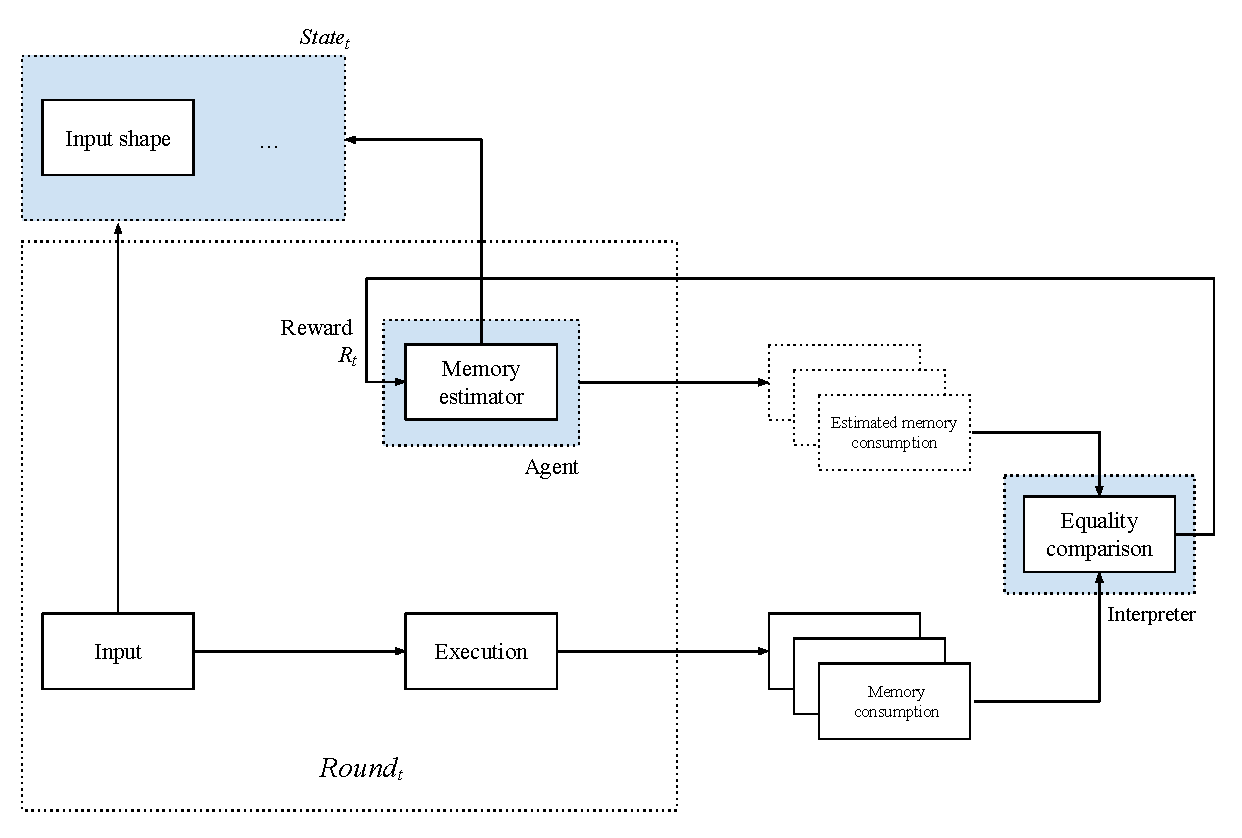
\includegraphics{usage-diagram.pdf}
  }
\end{figure}

\subsubsection{Python's garbage collection}

Python's garbage collector can pose a problem for us.
Python uses reference-counting as its garbage collection strategy, and it is lazy, so it usually waits for the memory to be needed to collect the garbage and free memory space.
If our operators are \ac{CPU} memory bounded, I may need to figure out how to deal with Python's garbage collector to gather the real memory usage when collecting memory consumption information to train the ML models.
However, I will only need to address this issue depending on the results of our experiments.

\subsubsection{Graph execution}

Another problem I may encounter is how to figure out the entire graph's memory requirements.
While our proposed solution can help us find the amount of memory required for a specific algorithm, integrating multiple algorithms into a graph poses a challenge.
I plan to address this issue by predicting not only the memory usage, but also the output shape of the algorithm and its features.
By having prior knowledge of the algorithms in the graph, I can compose a graph with the models using the output of the first model as the input data of the second one.
